\section{Generazione dei riferimenti variazionali a budget finito}
\label{app:oracle}

Per la campagna statica A, il campo gaussiano $u(\bm x)$ induce un funzionale di monitoraggio che penalizza la non uniformità della risoluzione rispetto al gradiente. La configurazione nodale $X$ è ottenuta minimizzando numericamente un funzionale $J(X;u)$ sotto il vincolo di bordo $\bm x_i=\bm x_i^{(0)}$ per $i\in B$ e la condizione di ammissibilità $J_e(X)\ge\varepsilon$ per ogni elemento. Le coordinate sono aggiornate sui nodi interni; la connettività rimane fissa.

I target sono generati con un budget finito di iterazioni quasi-Newton e accettati se il funzionale e l'errore d'interpolazione diminuiscono e la mesh resta ammissibile. La procedura produce riferimenti numerici riproducibili, ma non prova stazionarietà, ottimalità globale o convergenza dell'ottimizzatore. Questa distinzione è importante perché la GNN apprende una mappa verso gli spostamenti accettati, non una soluzione esatta di un problema di ottimizzazione certificato.

\begin{figure*}[!t]
\centering
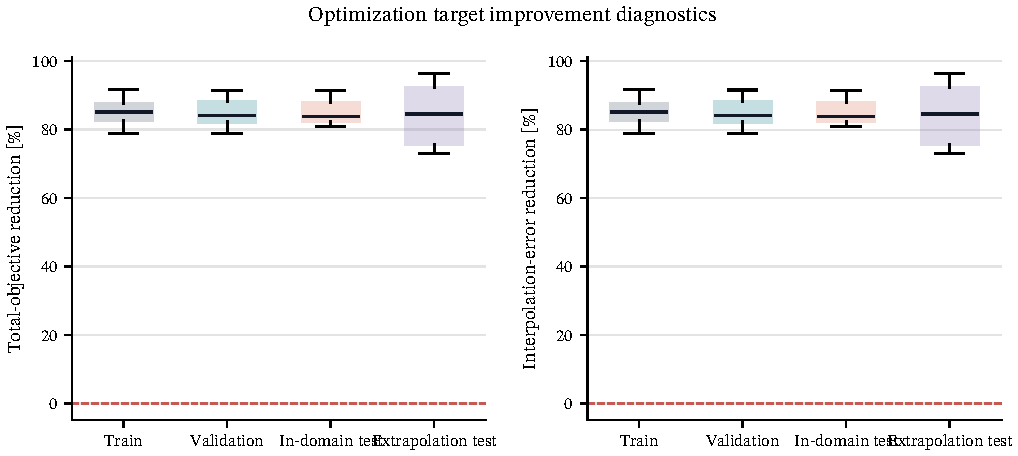
\includegraphics[width=0.78\textwidth,height=0.20\textheight,keepaspectratio]{images/appendix/dataset_target_improvement.pdf}
\caption{Riduzione del funzionale e dell'errore d'interpolazione associata ai riferimenti variazionali statici accettati.}
\label{fig:app_target_improvement}
\end{figure*}


